\documentclass[masters]{ucbthesis}
\usepackage[sorting=none]{biblatex}
\usepackage{amsmath}
\usepackage[version=3]{mhchem}
\usepackage{graphicx,subcaption}
\usepackage{listings}
\usepackage{hyperref}
\usepackage{multirow}
\usepackage{notoccite}
\usepackage[section]{placeins}
\hypersetup{
    colorlinks,
    citecolor=black,
    filecolor=black,
    linkcolor=black,
    urlcolor=black
}

% Double spacing, if you want it.
% \def\dsp{\def\baselinestretch{2.0}\large\normalsize}
% \dsp

% If the Grad. Division insists that the first paragraph of a section
% be indented (like the others), then include this line:
\usepackage{indentfirst}

\newtheorem{theorem}{Jibberish}

\bibliography{references}

\hyphenation{mar-gin-al-ia}

\setcounter{tocdepth}{3}

\makeatletter

\AtBeginDocument{%
     \expandafter\renewcommand\expandafter\subsection\expandafter
       {\expandafter\@fb@subsecFB\subsection}%
     \newcommand\@fb@subsecFB{\FloatBarrier
     \gdef\@fb@afterHHook{\@fb@topbarrier \gdef\@fb@afterHHook{}}}
     \g@addto@macro\@afterheading{\@fb@afterHHook}
     \gdef\@fb@afterHHook{}
  }

\begin{document}

% Declarations for Front Matter

\title{Delta-tracking in the GPU-accelerated WARP Monte Carlo Neutron Transport Code}
\author{Kelly L. Rowland}
\degreesemester{Spring}
\degreeyear{2015}
\degree{Master of Science}
\chair{Assistant Professor Rachel Slaybaugh}
\othermembers{Assistant Professor Massimiliano Fratoni \\ Professor Jasmina Vuji{\'c}}
\numberofmembers{3}
\prevdegrees{B.S. Rensselaer Polytechnic Institute 2013}
\field{Engineering - Nuclear Engineering}
\campus{Berkeley}

% For a masters thesis, uncomment (remove the % at the beginning of)
% the following line.  This affects the title and approval pages,
% which by default calls this a "dissertation", not a "thesis".

%\itsamasters

\maketitle
\approvalpage
\copyrightpage

\tableofcontents
\clearpage
\listoffigures
\clearpage
\listoftables

\begin{frontmatter}

\begin{acknowledgements}

\noindent This material is based upon work supported under an Integrated University Program Graduate 
Fellowship.
\\ \\
\noindent This work was partially supported by the Department of Energy National Nuclear Security 
Administration under Award Number(s) DE-NA0000979: The National Science and Security Consortium (NSSC), 
http://nssc.berkeley.edu/.

\end{acknowledgements}

\end{frontmatter}

\chapter{Introduction}

\section{Motivation}

Graphics processing units (GPUs) have gradually increased in computational power from small, 
job-specific boards to programmable powerhouses. Compared to more common central processing units (CPUs), 
GPUs have a higher aggregate memory bandwidth, much higher floating-point operations per second 
(FLOPs), and lower energy consumption per FLOP \cite{warp2015}.

As we approach exascale computing, many institutions are investing in GPU hardware to help achieve these
peak speeds. In the United States, Oak Ridge National Laboratory (ORNL) and Lawrence Livermore National
Laboratory (LLNL) are both acquiring high-performance computing systems that include NVIDIA GPU 
architectures \cite{ornl, llnl}. The computer system to be built at the Oak Ridge Leadership Computing
Facility will be named ``Summit" and will consist of nodes with multiple IBM POWER9 CPUs and NVIDIA Volta
accelerators. The architecture will use a coherent memory space that includes high bandwidth memory on the
GPUs and a high speed NVLink interconnect between the POWER9 CPU and Volta GPUs \cite{ornl}. ``Sierra",
the next advanced technology high-performance computing system to be introduced into LLNL's High
Performance Computing Complex, will also incorporate IBM POWER and NVIDIA Volta processors \cite{llnl}.
Additionally, it is estimated that Sierra will be about five times more power efficient than its
predecessor, Sequoia, while providing four to six times the sustained performance and five to seven times
the workload performance.

Supercomputing systems that use GPUs to accelerate computation are competitive in terms of speed when 
compared to other types of supercomputers. The TOP500 project uses a benchmark of ability to solve
linear systems of equations in dense matrix form to rank supercomputers. The most recent TOP500 list was
published in November 2014 \cite{top500} and demonstrated that supercomputers using GPU acceleration can
achieve peak speeds. The No.\ 2 and No.\ 6 systems both use NVIDIA GPUs to accelerate computation. 
Overall, fifty of the top 500 systems use NVIDIA chips for acceleration \cite{top500}.

However, transitioning to using these GPU-accelerated supercomputers will require substantial time
and effort. For many algorithms, CPU-optimized parallel algorithms are not directly portable to GPU 
architectures. In the field of nuclear engineering research and simulation specifically, neutral particle
transport codes must be rewritten to execute efficiently on GPUs \cite{warp2015}. In particular, the field
of nuclear engineering uses particle transport codes for reactor analysis, criticality safety, nuclear 
security and nonproliferation, detection, and shielding calculations.

Currently, there are not any general purpose Monte Carlo codes that execute on GPUs.
Two prominent codes used for neutron transport calculations in nuclear reactor analysis are the Monte
Carlo N-Particle (MCNP) code and the Serpent code. Both pieces of software use Monte Carlo methods to 
track neutron histories and perform criticality calculations on CPU-based computer architectures 
\cite{mcnp, serp_man}. At this time, however, there are no plans to adapt the MCNP code for use on GPUs
\cite{mcnp_nogpu}, providing incentive for nuclear engineering researchers to begin developing their own
Monte Carlo neutron transport software for efficient use on GPUs.

\section{WARP}

WARP, which can stand for ``Weaving All the Random Particles", is a three-dimensional (3D), continuous 
energy, Monte Carlo neutron transport code originally developed by Dr. Ryan M. Bergmann at UC Berkeley to 
efficiently execute on a CPU/GPU platform \cite{warp2015}. WARP is able to calculate multiplication 
factors, flux tallies, and fission source distributions for time-independent problems and can run in both 
criticality or fixed-source modes. WARP currently transports neutrons in unrestricted arrangements of 
spheres, cylinders, parallelpipeds, and hexagonal prisms \cite{warp2015} and is able to entertain both 
vacuum and reflecting (specular) boundary conditions.

What sets WARP apart from previous, somewhat similar endeavors is its breadth of scope and novel 
adaptation of the event-based Monte Carlo algorithm. Previous codes have been limited to restricted 
nuclear data or simplified geometry models, where WARP instead loads standard data files and uses a 
flexible, scalable, optimized geometry representation \cite{warp2015}. WARP uses a suite of 
highly-parallelized algorithms and employs a modified version of the original event-based algorithm that 
is better suited to GPU execution. For full detail, please see the paper by Bergmann and Vuji{\'c} (2015) 
\cite{warp2015}.

\chapter{Background}

\section{Delta-tracking theory}

The delta-tracking method was introduced by Woodcock in the 1960s. Although widely known, the method has
not been commonly used as the primary transport method in general purpose Monte Carlo codes, probably 
because of its limitations discussed below \cite{serp_delta}.

In Monte Carlo neutron transport, we track anything that can happen to neutrons in a system: collisions 
and their outcomes, surface crossings, etc. To do that, we need to track how these particles move in that 
system. This starts with determining the number of path lengths they cover between events.
The number of path lengths traveled by a given neutron is sampled from an exponential distribution using

\begin{equation}
\ell = \frac{-\log\xi}{\Sigma_{\mathrm{tot,m}}(E)},
\end{equation}

\noindent where $\xi$ is a uniformly-distributed random variable on the unit interval and 
$\Sigma_{\mathrm{tot,m}}$ is the macroscopic total cross section of the material $m$ in which the neutron 
is located. The total cross section characterizes the neutron collision probability per unit path length 
traveled in the medium.

However, the sampled path length is not statistically valid if the neutron crosses a material boundary; 
the flight is stopped at the boundary surface and a new path length is sampled with the new material total
cross section. This is the main principle of conventional ray tracing \cite{serp_delta} and is what is
done in WARP with the OptiX framework, as discussed below.

The idea behind delta-tracking is to effectively homogenize the total cross sections such that the sampled
path lengths are valid over the entire geometry. Consider the concept of the ``virtual collision", a 
scattering reaction that preserves neutron energy and direction. Since virtual collisions have no impact 
on the final outcome, any number of them can ``happen" in the random walk. Therefore, the total cross 
section of a material can be adjusted by adding an arbitrary virtual collision cross section, 
$\Sigma_\mathrm{{0,m}}(E)$
\cite{serp_delta}:

\begin{equation}
\Sigma'_{\mathrm{tot,m}}(E) = \Sigma_{\mathrm{tot,m}}(E) + \Sigma_\mathrm{{0,m}}(E).
\end{equation}

Because all material cross sections can now be freely and arbitrarily increased, a \textit{majorant} cross
section can be assigned to represent the effective total (physical + virtual) collision probability in all
materials along a given neutron's trajectory:
\begin{equation}
\label{eq:maj}
\begin{aligned}
\Sigma_{\mathrm{maj}}(E) &= \Sigma'_{\mathrm{tot,1}}(E) = \Sigma'_{\mathrm{tot,2}}(E) = \ldots = 
\Sigma'_{\mathrm{tot,M}}(E) \\
& = \max\{\Sigma_{\mathrm{tot,1}}(E), \Sigma_{\mathrm{tot,2}}(E), \ldots, \Sigma_{\mathrm{tot,M}}(E)\}\:,
\end{aligned}
\end{equation}
where $M$ is the number of materials along a neutron's flight path.

Path lengths sampled using the global majorant are statistically valid in all materials, effectively
homogenizing the material total cross sections and eliminating the need to calculate surface intersection
distances \cite{serp_delta}. Instead, an additional step is included in the tracking routine for handling 
virtual collisions. Rejection sampling is carried out for each collision, and the collision point is 
accepted with probability 

\begin{equation}
P_{\mathrm{col}}(E) = \frac{\Sigma_{\mathrm{tot,col}}(E)}{\Sigma_{\mathrm{maj}}(E)}. 
\end{equation}

\noindent If the point is rejected, the collision is considered virtual and the random walk continues by 
sampling a new path length.

The inherent advantage of delta-tracking is that the neutron random walk can be continued over material
boundaries without stopping the walk at each surface crossing. The geometry routine reduces to
determining the material in which the collision point resides, which is computationally less expensive 
than calculating the surface distances when running a simulation on traditional CPU hardware 
\cite{serp_delta}. The simplified geometry routine is advantageous in that delta-tracking is often faster 
than ray tracing in complex geometries, and complicated objects and surface types are easier to handle 
with a delta-tracking algorithm \cite{serp_delta}.

One shortcoming of the delta-tracking method arises when material total cross sections differ greatly. A
representative example of this is a light water reactor (LWR) fuel assembly that contains localized heavy 
absorbers (such as control rods or burnable poison rods) \cite{serp_delta}. Although the absorber itself
occupies a relatively small space physically, its large cross section dominates the majorant at low 
neutron energies. This causes the neutron random walk to be cut into many short tracks, wasting computing
time by continually incurring virtual collisions and resampling. 

Additionally, using the delta-tracking method necessitates the use of the collision flux estimator rather 
than the track-length flux estimator, which is generally considered a drawback for implementation in 
traditional Monte Carlo codes \cite{serp_delta}. The track-length estimation of the reaction rate integral
can be written in simplest analog form as

\begin{equation}
R_{\mathrm{tle}} = \sum_{i=1}^{I}\ell_{i}f_{i},
\end{equation}

\noindent where $\ell$ is the neutron track length, $f$ is the response function, and the summation is 
over all tracks in the region of interest. This estimator cannot be used when employing the delta-tracking
method because the sampled neutron paths may extend over several material regions and the discontinuity
points are not known \cite{serp_delta}. 

An alternative to the track-length flux estimator is the collision flux estimator:

\begin{equation}
R_{\mathrm{cfe}} = \sum_{i=1}^{I}\frac{f_i}{\Sigma_{\mathrm{tot,i}}},
\end{equation}

\noindent where $\Sigma_{\mathrm{tot}}$ is the material total macroscopic cross section at the collision 
site and the summation is over all collisions within the region of interest \cite{serp_delta}. This flux 
estimator is problematic in that it often results in poor efficiency for tallies scored in regions of low 
volume or with low collision density. However, the use of the collision flux estimator should not be 
considered a disadvantage for the implementation of the delta-tracking method in WARP; this estimator is 
already the code's flux tally method \cite{warp2015}.

In WARP, the flux tally kernel scores collisions in cell $j$ with volume $V_j$ as shown in Equation 
\ref{tally}, where $\Sigma_{\mathrm{tot,j}}(E)$ is the total macroscopic cross section at energy 
$E_i < E < E_{i+1}$ and $N_{i,j}$ is the number of collisions in that volume \cite{warp2015}:

\begin{equation}
\label{tally}
\bar{\phi}_{i,j} = \frac{1}{V_j}\sum_{i=1}^{N_{i,j}}\frac{1}{\Sigma_{\mathrm{tot,j}}(E)}\:.
\end{equation}

\section{Ray tracing in WARP}
\label{sec:rt}

WARP uses the NVIDIA OptiX ray tracing framework for geometry representation \cite{warp2015}. OptiX is a
highly-optimized, scalable framework developed by NVIDIA for building ray tracing-based applications. It
allows for user-written applications that use ray tracing for graphics, collision detection, and other
fields of interest \cite{optix_man}; the flexibility of the framework makes it suitable for this 
application in Monte Carlo neutron transport. The OptiX engine is composed of a host-based API that 
defines ray tracing based data structures, which works in combination with a CUDA C-based programming 
system that can produce new rays, intersect rays with surfaces, and respond to those intersections 
\cite{optix_man}.

In WARP and other Monte Carlo codes that use ray tracing to track particle locations, material information
is updated when a sampled interaction distance is greater than the nearest surface distance. The neutron 
is moved to the boundary that it will cross, the material information is updated to the material that the 
neutron is entering, and the interaction distance is resampled in the new material using the same 
direction of flight \cite{warp2015}. WARP uses an algorithm that uses the OptiX framework to perform the 
ray tracing required to determine the entering material. Since all of the system geometric information is 
stored in the OptiX context \cite{warp2015}, this allows the material information update to be done 
readily. 

WARP represents geometric volumes as the intersection of the space inside of a given cell with the space
outside any cells that are nested inside of it \cite{warp2015}. For example, if two objects were 
designated to be centered at the same coordinate point with the inner object entirely encompassed by the 
outer object, the space between the two objects would belong to the outer object while the volume inside 
of the inner object would all belong to the inner object. This is important to note because it sets the
type of algorithms that can be used for geometry handling.

WARP's material query algorithm is shown in Figure \ref{whereami} \cite{warp2015}. A list of surface
intersections, ordered by proximity, is generated by iteratively ray tracing along a neutron's direction
of flight and adding the closest surface number to the hit list each time. Tracing is stopped once the
ray hits a predefined outer cell that contains all other cells \cite{warp2015}. Because all surfaces are
closed, the ray intersects any cell surface twice if its origin is not nested in the cell in which the ray
originated. When the list of surface intersections is created, the double entries are removed, resulting 
in a list of cells in which the neutron is nested. The first entry of the list is the cell in which the 
neutron is located at the time of the material query and the second entry of the list is the cell that the
neutron is entering \cite{warp2015}.

\begin{figure}[h!] 
  \centering
    \includegraphics[width=1.0\textwidth]{img/whereami.eps}
     \caption{The point-in-polygon-like algorithm for determining the entering cell/material number by 
		using ray tracing. \label{whereami} }
\end{figure}

One particular issue with ray tracing is that cell descriptions are mathematically exact, but they are
represented by inexact numbers. Floating-point roundoff can cause a neutron to be placed slightly behind
a boundary instead of at the actual boundary. This situation can largely be prevented by using an OptiX 
scene ``epsilon", which designates the minimum distance away from the source point at which intersections 
are allowed to occur \cite{warp2015}. The scene epsilon helps ensure that a trace starts after a boundary
such that accurate results are calculated. For the algorithm to be used effectively, it is important that
the scene epsilon is set to an appropriate value for the problem geometry \cite{warp2015}.

The scene epsilon, however, can also cause inaccurate material queries in certain geometry configurations.
If the thickness of an intersected object is less than the scene epsilon, the material query algorithm may
only count a single intersection of the object instead of two. The code will then assign the neutron the 
thin object's material rather than determining that the neutron moved through the thin material and into the subsequent one \cite{warp2015}. In many cases, this can be avoided by performing the
surface intersection in the direction of the neutron flight path and then performing the material query in
the z-direction only. At this point in development, the objects in WARP are all z-aligned, optically
thick shapes. Thus, the previously described incorrect material query will not happen if the material 
query is done in the z-direction because the ray will only intersect planes perpendicular to it 
\cite{warp2015}.

An additional issue that can occur in using this algorithm happens when cells have coincident surfaces. In
this case, the number of the cell that is actually intersected is undefined and the following trace 
iteration will skip the intersection of the coincident cell. One way to avoid this would be to ensure that
coincident surfaces are more than one scene epsilon apart \cite{warp2015}. In some cases, the
neutron mean free path is significantly larger than this introduced gap and this approximation will not
affect the results. However, if the mean free path is smaller than the gap (which may happen in cells next
to strong absorbers), errors could be introduced by the approximation. An automatic way of determining
this may be an area of future development in WARP \cite{warp2015}. 

\section{Delta-tracking in existing Monte Carlo neutron transport codes}

Over the years, many codes have had delta-tracking available as at least an option for neutron tracking. 
We will point out, however, that none of these codes were implemented on GPUs. 

The concept of delta-tracking was introduced in the ``HOLE" routines in the GEM code, which was designed 
to study criticality safety problems in chemical plants with the primary objective of using nuclear data 
in the finest detail as was possible \cite{wc}. Subsequent developments in the code enabled calculations 
that included all significant structural features of a complete reactor.

Geometric representation in GEM was similar to that in WARP, discussed above. The system was divided into
regions by boundaries that form closed, nested surfaces that can touch or coincide but cannot intersect.
Regions filled by a single homogeneous material were specified only by their atomic composition and 
density, while the geometry of a heterogeneous region was handled with the delta-tracking method in the
HOLE routine \cite{wc}. This method was used to reduce the mean free path of all materials in the region
to the same value such that they were independent of internal boundaries.

RCP01, a Monte Carlo program used to analyze geometries of interest in nuclear design and analysis of LWRs
and their associated technologies, used delta-tracking as an optional acceleration method \cite{rcp01}.
``Fast" tracking in subcell regions could be turned on by the user; this switched on delta-tracking based 
upon the maximum cross section in the subcell. This method could not be used in conjunction with point 
detectors.

Delta-tracking was also an optional feature in RACER, a system of codes used for Monte Carlo nuclear 
reactor physics analysis \cite{racer}. The ``Monte Carlo - Vectorized" (MCV) module offered the option of
using the delta-tracking method on the basis that it is potentially more efficient than ``regular" 
tracking in some instances. The user needed to specify the tracking scheme for each neutron tally group, 
resulting in the overall use of a mixed tracking scheme that varied with neutron energy. This was 
necessary for both consistent tally estimation and efficient neutron tracking.

The ``MCU-PD" version of the Monte Carlo Universal code uses the option of delta-tracking for geometry 
simplification \cite{mcu}. Systems in MCU-PD are represented as unions of homogeneous geometric areas, 
each described as a boolean combination of a set of simple bodies (that is, the code uses the method of 
combinatorial geometry). One limitation of the method of combinatorial geometry is that complex boundary
surfaces must be approximated by a large number of zones. In MCU-PD, use of the delta-tracking method
removes this limitation. 

The VMONT code is a fuel assembly analysis code that uses a vectorized Monte Carlo method for neutron 
transport calculation and incorporates delta-tracking to decrease code runtime and processing 
\cite{vmont}. It was found in this code that without delta-tracking, neutron flight path analysis took up
about 80\% of computing time; implementation of delta-tracking resulted in a speedup factor of 1.5
relative to this figure.

MONK, a Monte Carlo neutronics code for the solution of criticality safety and reactor physics problems,
has its origins in the GEM code discussed above. Along with the Monte Carlo code MCBEND, MONK is part of
the ANSWERS codes suite, which is used for calculations involving a variety of reactor types, including
experimental reactors \cite{mcbend}. Both codes use a common geometry package containing the component
``Hole Geometry", which uses delta-tracking. Hole Geometry is complementary to the conventional ray 
tracing ``Fractal Geometry"; the Hole Geometry package facilitates exact modeling of complicated geometry
configurations that would be impossible to model using the simple bodies in the Fractal Geometry package.

Delta-tracking is an option in the MORET 5 code, a Monte Carlo code designed to perform calculations to
support criticality safety assessments \cite{moret}. MORET 5 uses a combinatorial geometry scheme and
allows use of delta-tracking to reduce runtime in scenarios involving complex geometries, especially those
with complex shapes or that have a large number of volumes with dimensions smaller than the neutron mean
free path (such as a pebble bed reactor).

The Serpent Monte Carlo reactor physics burnup calculation code employs a unique combination of both ray
tracing and delta-tracking in its geometry routine. The code originally used only the delta-tracking 
method, which was chosen for the sake of simplicity, but efficiency problems induced by the presence of 
heavy localized absorbers when using the delta-tracking method led to the hybrid geometry method currently
used in Serpent \cite{serp_thesis}.

Serpent switches to using ray tracing when collision sampling efficiency is low. Selection between the two
methods is done by comparing the neutron mean free path resulting from the majorant to the physical value 
of the mean free path given by the material total cross section at the neutron's location 
\cite{serp_delta}. If
%
\begin{equation}
\label{deltaray}
\frac{\ell_{\mathrm{maj}}(E)}{\ell_m(E)}=\frac{\Sigma_{\mathrm{tot,m}}(E)}{\Sigma_{\mathrm{maj}}(E)}>1-c,
\end{equation}
%
where $\ell_m$ is the material-calculated path length and $\ell_{\mathrm{maj}}$ is the majorant-calculated
path length, the neutron path length is sampled using the majorant cross section and rejection sampling is
subsequently carried out at the collision point. The constant $c$ is the predefined cutoff criterion 
valued between 0 (no delta-tracking) and 1 (no ray tracing). After several parametric studies were 
performed to assess the runtime of the Serpent code for different reactor geometries with varied values of
$c$, the cutoff criterion value was set to a default fixed value of 0.90 \cite{serp_delta} but can be 
changed by the user.

The Serpent parametric studies also compared the flux estimates in two of the LWR lattice configurations 
to demonstrate that the decrease in runtime from the use of the delta-tracking method is not outweighed by
poor statistics. Comparisons were done with the figure-of-merit (FOM) metric, defined below, which 
incorporates both the calculation time $T$ and the relative statistical error $\Delta x/x$ of the result 
\cite{serp_delta}. 

\begin{equation}
\label{fom}
\text{FOM} = \frac{1}{T(\Delta x/x)^2}
\end{equation}

It was found that, for parameters integrated over the entire geometry, the accuracy of the two methods is 
comparable.

\section{Vector computing as a basis for GPU algorithims}

The origin of the ideas in WARP is research done in the 1980s and 1990s for mapping the Monte Carlo and 
collision probability methods onto vector computers \cite{warp2015}. These methods on those machines used 
an ``event-based" algorithm in which neutrons are organized and processed according to their required 
operation. If a neutron is about to undergo inelastic scattering, its data are put into the inelastic 
scattering buffer. The same process is done for all reaction types: neutrons inducing fission are placed 
in the fission buffer, and so on. Vector processing calculations such as these are more generally referred
to as ``single instruction multiple data", or SIMD, processes. Since GPUs are massively parallel and rely 
on SIMD, the WARP code uses a modified event-based algorithm for GPU-accelerated Monte Carlo neutron 
transport.

The RACER and VMONT codes were both vectorized Monte Carlo codes that used delta-tracking for the purpose 
of reducing runtime and processing. It follows logically that, since delta-tracking has been shown to be 
efficient in these vector machine codes, it has the potential to be efficient when used on a 
GPU-accelerated, vectorized Monte Carlo code such as WARP.


\chapter{Implementation}

\section{Delta-tracking in WARP}

The implementation of delta-tracking in WARP is somewhat similar to the implementation in RACER and 
Serpent in that it uses a combination of ray tracing and delta-tracking. 
To understand what is happening in WARP, what follows is an explanation of the general delta-tracking 
algorithm implemented, a comparison to ray tracing, discussion of the specific implementation in WARP, and
finally some comments about the performance potential of using delta-tracking on GPUs for the first time.

In WARP, the delta tracking algorithm executes these steps:

\begin{itemize}
	\item{get current neutron positions using OptiX trace;}
	\item{calculate majorant cross section, sample path lengths, update neutron coordinates;}
	\item{update neutron positions and material information using OptiX trace;}
	\item{calculate material total cross section and perform rejection sampling;}
	\item{determine neutron interaction.}
\end{itemize}

\noindent For direct comparison, tracking particles via ray tracing only in WARP is executed as:

\begin{itemize}
	\item{get current neutron positions using OptiX trace;}
	\item{calculate macroscopic total cross section and sample path length;}
	\item{determine with which isotope neutron interacts;}
	\item{move neutron to collision site or cell boundary, whichever is closer;}
	\item{determine neutron interaction.}
\end{itemize}

\noindent From there, with either tracking scheme, neutrons are grouped based on the interactions that 
they are about to undergo and the vectors are subsequently processed.

\section{Implementation}

In WARP and other Monte Carlo neutron transport codes, particle positions are updated as:

\begin{gather}
\label{eq:move}
x \mathrel{+}= \ell\hat{x}, \nonumber\\
y \mathrel{+}= \ell\hat{y}, \\
z \mathrel{+}= \ell\hat{z}, \nonumber
\end{gather}

\noindent where $\ell$, the sampled travel distance is defined as:

\begin{equation}
\ell = 
	\begin{cases}
	\frac{-\log\xi}{\Sigma_{\mathrm{tot}}} & \text{with ray tracing}, \\
	\frac{-\log\xi}{\Sigma_{\mathrm{maj}}} & \text{with delta-tracking}. \\
	\end{cases}
\end{equation}

If ray tracing is being used, a check is performed between the sampled neutron flight distance and the
distance to the nearest boundary crossing on that trajectory. If the boundary crossing is closer than the
sampled distance, the particle position is instead updated as

\begin{gather}
x \mathrel{+}= s\hat{x} + \varepsilon x_{\mathrm{norm}}, \nonumber\\
y \mathrel{+}= s\hat{y} + \varepsilon y_{\mathrm{norm}}, \\
z \mathrel{+}= s\hat{z} + \varepsilon z_{\mathrm{norm}}, \nonumber
\end{gather}

\noindent where $s$ is the distance to the surface to be crossed. The epsilon term added to the position 
is required
by the use of the OptiX framework; the inclusion of this term ensures that the neutron is sufficiently far
 into the new cell such that it can be detected by OptiX and the corresponding material updated
accordingly. The second term uses vector norms rather than the vector directions in Equation \ref{eq:move}
to move particles away from the surface in a perpendicular manner rather than potentially along a surface
boundary (which could cause issues with OptiX detection). In this case of a particle crossing a boundary
with ray tracing, the particle is stopped at this updated location and the flight path distance must be
resampled using the total macrscopic cross section of the new material.

Although delta-tracking circumvents the above resampling in the case of surface crossings, there is a 
potential need to resample at each collision site. The collision site is accepted as an actual reaction 
with probability

\begin{equation}
P_{\mathrm{col}}(E) = \frac{\Sigma_{\mathrm{tot,col}}(E)}{\Sigma_{\mathrm{maj}}(E)} 
\end{equation}

\noindent and rejected as a ``virtual" collision otherwise. It is important to note that this rejection
sampling must use the total macrscopic cross section of the material in which the collision is being 
considered and not the material in which the neutron was originally located. If the collision is 
considered virtual, a new path length is sampled with the majorant cross section again, and the transport
process continues.

It should be noted that calculating the majorant cross section in WARP is done na{\"i}vely:

\begin{equation}
\label{eq:majnaive}
\Sigma_{\mathrm{maj}}(E)
= \max\{\Sigma_{\mathrm{tot,1}}(E), \Sigma_{\mathrm{tot,2}}(E), \ldots, \Sigma_{\mathrm{tot,M}}(E)\}\:,
\end{equation}

\noindent where $M$ is the number of materials in the entire system. One potential area of development 
would be to
calculate the majorant cross section along the neutron's trajectory (as specified in Equation 
\ref{eq:maj}) rather than this ``global" majorant cross section.

With either tracking method, once the neutron has been determined to undergo an actual collision the 
reaction it will experience is chosen using the microscopic cross sections of the material in which 
the particle is located. Following this, the reaction is processed, and transport continues as above.

\section{Performance potential of delta-tracking in WARP}

Because the OptiX trace must be done twice in each instance of the delta-tracking process and the origina 
ray tracing method only necessitates one trace, it may be that the current implementation of 
delta-tracking may not result be faster than standard ray tracing for simple geometry and 
material configurations. It has been seen in various other Monte Carlo neutron
transport codes that the bulk of the runtime is involved with ray tracing, and WARP is not too different
from other codes in that regard.
This issue could potentially be circumvented if a different framework were to be used rather than OptiX,
but this would require a sizable overhaul of the code and was not considered for this
project. Further, the OptiX framework is optimized for NVIDIA GPUs and at this time it is unclear what
a new, better choice might be. 

However, it is expected that, like in other codes, delta-tracking may be more efficient in WARP when
considering certain geometry configurations. Like Serpent, WARP is intended for calculations in nuclear
reactor analysis. Many reactor configurations consist of lattices composed of many geometry and material
boundaries, causing simulations that use ray tracing to run slowly because 
neutron flights stop at each boundary crossing. Thus, the time saved in not stopping neutron
flights at boundary crossings may compensate for having to call an additional OptiX trace in the 
delta-tracking method implemented in WARP.


\chapter{Results}

The question that this research is answering is whether this expected behavior of delta-tracking,
which is to perform within statistical accuracy to ray tracing with lower runtime, holds on GPUs compared 
to CPUs. The expected behavior is of interest because it is crucial to the study that results are 
statisically accurate; runtime is irrelevant if the calculations are performed incorrectly. Additionally, 
it is of interest to developers to see if delta-tracking is faster than ray tracing on an advanced 
computer architecture.

The problems investigated here 
are designed to answer these questions by testing a variety of problems relevant to reactor physics, 
ranging from very simple systems comprised of one cell and one isotope to a complex configuration of
hundreds of cells and multiple isotopes.
This strategy allows detailed investigation of the algorithm as well as demonstrating behavior for 
problems of interest.

Here, the version of WARP with delta-tracking is compared against the version of WARP with ray tracing.
The original ray tracing version of the code has been benchmarked against both MCNP and Serpent 
\cite{warp_thesis} so, for this work, it is sufficient to assess how well results from the delta-tracking 
version of WARP match those generated by the ray tracing version. The success criteria of the 
delta-tracking version of WARP will be whether the results are statistically accurate compared to the ray
tracing version of WARP and if the calculation time is lower than the ray tracing version of WARP.

As WARP is still in development, it currently only supports four geometry and material configurations.
These configurations can be lumped into two groups: homogeneous systems and heterogeneous systems. The 
geometry parameters for the four configurations are listed in Table \ref{test_setup} \cite{warp2015}. The
pin cell and assembly cases contain water at 3 g/cm$^3$, which was an error introduced in the original
calculations \cite{warp_thesis}.
We have retained this water density so we can make direct comparisons. 
 Although this is clearly unphysical, it does not have an impact 
on the simulation results and, since both versions of WARP contain the same geometry configurations, the 
comparisons are consistent.

\begin{table}[h]
\centering
\caption{Geometry and materials used in the test cases.}
\label{test_setup}
\begin{tabular}{| c | c | c | c | c |}
 \hline
 \textbf{Test} & \textbf{Number and Type of Cells} & \textbf{Material(s)} & \textbf{Isotope(s)} & 
\textbf{Density} \\
 \hline
 Jezebel & 1 sphere; r = 5.1cm & Fuel & (1.00) $^{239}$Pu & 19.816 g/cm$^3$\\
  \hline
 \multirow{3}{*}{Homogenized}  & \multirow{4}{*}{1 cube; r = 10cm } & \multirow{4}{*}{Hom. Fuel} & (0.90) $^{238}$U  & \multirow{4}{*}{10  g/cm$^3$} \\
  \multirow{3}{*}{Block} & & & (0.10) $^{235}$U & \\
 & & & (3.00) $^{16}$O   & \\
 & & & (2.00) $^{1}$H     & \\
  \hline
 \multirow{5}{*}{Pin Cell}                        & \multirow{4}{*}{1 cuboid, 10x10x50cm} & \multirow{3}{*}{Fuel} & (0.90) $^{238}$U & \multirow{3}{*}{15  g/cm$^3$} \\
 &  \multirow{4}{*}{1 cylinder; r = 1cm, z = 40cm} & & (0.10) $^{235}$U & \\
  & & & (2.00) $^{16}$O & \\
 \cline{3-5}
 & & \multirow{2}{*}{Water} & (1.00) $^{16}$O &  \multirow{2}{*}{3  g/cm$^3$} \\
 & & & (2.00) $^{1}$H & \\
  \hline
  \multirow{5}{*}{Hex Assembly}  & \multirow{4}{*}{1 cube, 84cm$^3$} & \multirow{3}{*}{Fuel} & (0.90) $^{238}$U & \multirow{3}{*}{15  g/cm$^3$} \\
   & \multirow{4}{*}{{\small 631 cylinders; r = 1cm, z = 40cm}} & & (0.10) $^{235}$U & \\
     & & & (2.00) $^{16}$O & \\
 \cline{3-5}
 & & \multirow{2}{*}{Water} & (1.00) $^{16}$O &  \multirow{2}{*}{3  g/cm$^3$} \\
 & & & (2.00) $^{1}$H & \\
  \hline
 \end{tabular}
\end{table}

All calculations were performed on an NVIDIA GeForce GTX TITAN Black graphics card. Additionally, the 
following results all use these particular specifications:
	\begin{itemize}
	\item{500 000 neutron histories,}
	\item{20 inactive cycles followed by 40 active cycles,}
	\item{vacuum boundary conditions, and}
	\item{Serpent ENDF/B-VII ACE data at 300K.}
	\end{itemize}

For each of the configurations, it is expected that the delta-tracking version of WARP will arrive at a
statistically accurate calculation of the system's effective multiplication factor and that the neutron 
flux spectra generated by both versions of the code will be consistent. Additionally, it is expected that,
for calculations involving homogeneous systems, the delta-tracking version of WARP will be slower than
those performed with the ray tracing version of WARP. This is because, compared to the ray tracing 
routine, the delta-tracking routine requires an additional OptiX trace to update neutron locations after 
the particles have been moved. This is done in order to retrieve the updated material information required
for the rejection sampling incurred in delta-tracking. We conduct homogeneous system comparisons in order
to verify algorithm correctness. For the heterogeneous systems, it is expected that
the delta-tracking version of WARP may be faster than the ray tracing version; not stopping the neutrons
at each boundary crossing may save more time than is induced by the extra neutron position updates.

\section{Homogeneous systems}
\label{sec:homog}

The delta-tracking method was first tested in the two homogeneous systems to ensure that the method
delivers accurate results compared to those in the original version of the code. It was expected that the
calculated results would be accurate within statistical error but that the calculations performed using
delta-tracking would be slower than those performed with ray tracing. Because there is only one cell and
therefore one boundary in these systems, delta-tracking should not have any advantage over ray tracing as
ray tracing is still used to check whether or not a neutron has leaked out of the system. Additionally,
the delta-tracking method requires the code to do an extra update of neutron position when compared to the
ray tracing algorithm, and it is expected that these supplementary calculations will incur more runtime.

\subsection{Bare plutonium sphere}

The ``Jezebel" test is a bare plutonium sphere and is considered to be a standard criticality test 
\cite{nea1995}. The actual geometry configuration is a sphere of plutonium-239 with a radius of 5.1 cm.
Computational results for the Jezebel scenario are shown in Table \ref{pu_table} and Figure \ref{jezebel}.

\begin{table}[h!]
\centering
\caption{Calculated multiplication factors and runtimes for the Jezebel configuration.}
\label{pu_table}
\begin{tabular}{| c | c | c |}
\hline
\textbf{Method} & $\mathbf{k_{\mathrm{eff}}}$ & \textbf{Runtime} \\
\hline
Ray tracing & $1.027853 \pm 3.8304 \times 10^{-4}$ & 16.17 s \\
Delta-tracking & $1.026794 \pm 3.5830 \times 10^{-4}$ & 22.73 s \\
\hline
\end{tabular}
\end{table}

\begin{figure}[h!]
\includegraphics[width=\textwidth]{img/godiva.eps}
\caption{Normalized flux spectra for the Jezebel configuration generated by both versions of WARP.
\label{jezebel}}
\end{figure}

The multiplication factors calculated by each method match within statistical uncertainty and the flux
spectra are nearly (if not actually) identical. The runtimes are comparable for both 
methods. Here, it should not be expected that the delta-tracking method would be considerably different 
compared to the ray tracing algorithm, as the system only contains one cell with one material composed of 
a single isotope.

\subsection{Homogenized block}

The ``homogenized block" test consists of one cube with edges 20 cm in length. The cube is composed of a
homogeneous mixture of 10\% $\ce{^{235}U}$ enriched $\ce{UO_2}$ and water at a 1:1 ratio \cite{warp2015}.
While still a homogeneous case, the homogeneous block is more complex than the Jezebel scenario in that
its single material is composed of multiple isotopes. We are again testing that the delta-tracking
method calculates accurate results, but it is expected that the extra calculations involved in determining
the majorant cross section and the extra OptiX trace needed in the delta-tracking routine will cause an 
increase in runtime. Results for the homogenized block configuration are shown in Table \ref{hom_table} 
and Figure \ref{homfuel}.

\begin{table}[h!]
\centering
\caption{Calculated multiplication factors and runtimes for the homogenized block configuration.}
\label{hom_table}
\begin{tabular}{| c | c | c |}
\hline
\textbf{Method} & $\mathbf{k_{\mathrm{eff}}}$ & \textbf{Runtime} \\
\hline
Ray tracing & $1.213833 \pm 2.9255 \times 10^{-4}$ & 28.14 s \\
Delta-tracking & $1.213983 \pm 2.1413 \times 10^{-4}$ & 30.51 s \\
\hline
\end{tabular}
\end{table}

\begin{figure}[h!]
\includegraphics[width=\textwidth]{img/homfuel.eps}
\caption{Normalized flux spectra for the homogenized block configuration generated by both 
versions of WARP. \label{homfuel}}
\end{figure}

Again, the multiplication factor calculated by the delta-tracking version of WARP matches that calculated
by the ray tracing version of WARP (within statistical error). The flux spectra are also consistent with
one another. However, this case shows a greater discrepancy in the runtimes of each of the two methods. 
The version of the code that uses the delta-tracking method is considerably slower, likely because of the
extra calculations required to compute the majorant cross section and the additional OptiX trace required 
in each run.

\section{Heterogeneous systems}
\label{sec:hetero}

For the heterogeneous systems, we are once again testing that the delta-tracking method produces results
that are statistically accurate compared to results calculated using the ray tracing algorithm. However,
for these systems it is expected that the delta-tracking method may be faster than the ray tracing
algorithm. Although additional calculations are incurred in the determination of the majorant cross
section and the additional OptiX trace required for the delta-tracking routine, the time saved in not 
having to stop neutrons at each material boundary may be enough to result in a reduction in runtime with 
the use of the delta-tracking method.

\subsection{Fuel pin cell}

The ``pin cell" test contains a bare $\ce{UO_2}$ cylinder encased in a block of water. The pin has a 
diameter of 1 cm and a length of 40 cm; the dimensions of the surrounding water block are 10 $\times$ 10
$\times$ 50 cm \cite{warp2015}. This test has two materials, each with multiple isotopes, and two cells.
Results can be seen in Table \ref{pin_table} and Figures \ref{pincell-fuel} and \ref{pincell-water}.

\begin{table}[h!]
\centering
\caption{Calculated multiplication factors and runtimes for the pin cell configuration.}
\label{pin_table}
\begin{tabular}{| c | c | c |}
\hline
\textbf{Method} & $\mathbf{k_{\mathrm{eff}}}$ & \textbf{Runtime} \\
\hline
Ray tracing & $3.798339 \times 10^{-1} \pm 6.3999 \times 10^{-4}$ & 3.66683 min \\
Delta-tracking & $3.822616 \times 10^{-1} \pm 4.9758 \times 10^{-4}$ & 3.703 min \\
\hline
\end{tabular}
\end{table}

\begin{figure}[h!]
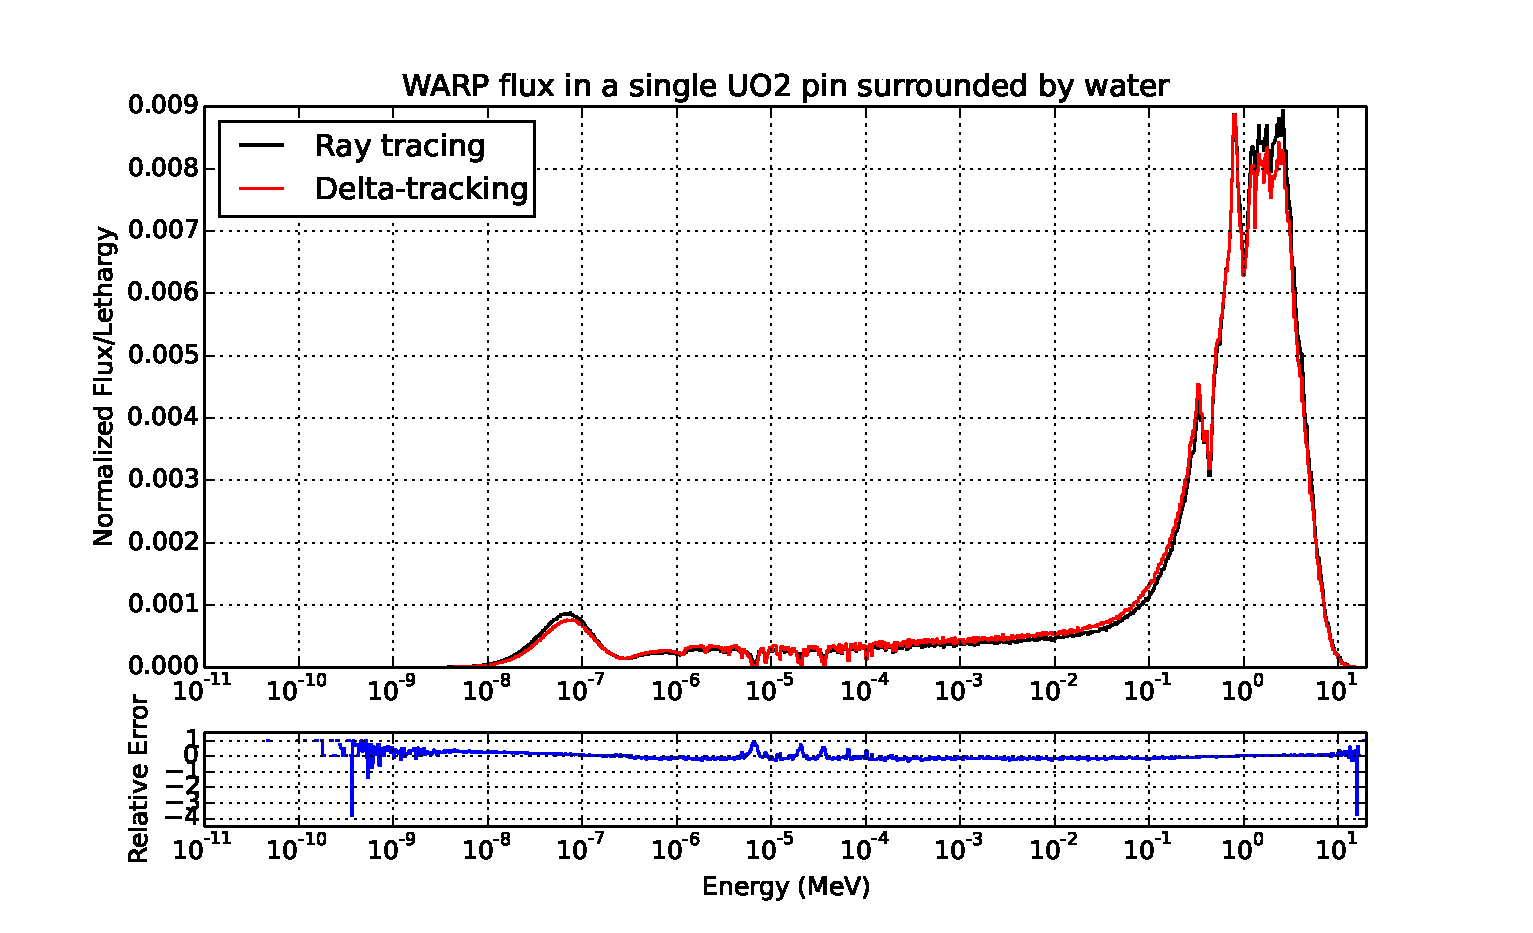
\includegraphics[width=\textwidth]{img/pincell-fuel.eps}
\caption{Normalized flux spectra for the \textbf{$\ce{UO_2}$ cylinder} in the pin cell 
configuration generated by both versions of WARP. \label{pincell-fuel}}
\end{figure}

\begin{figure}[h!]
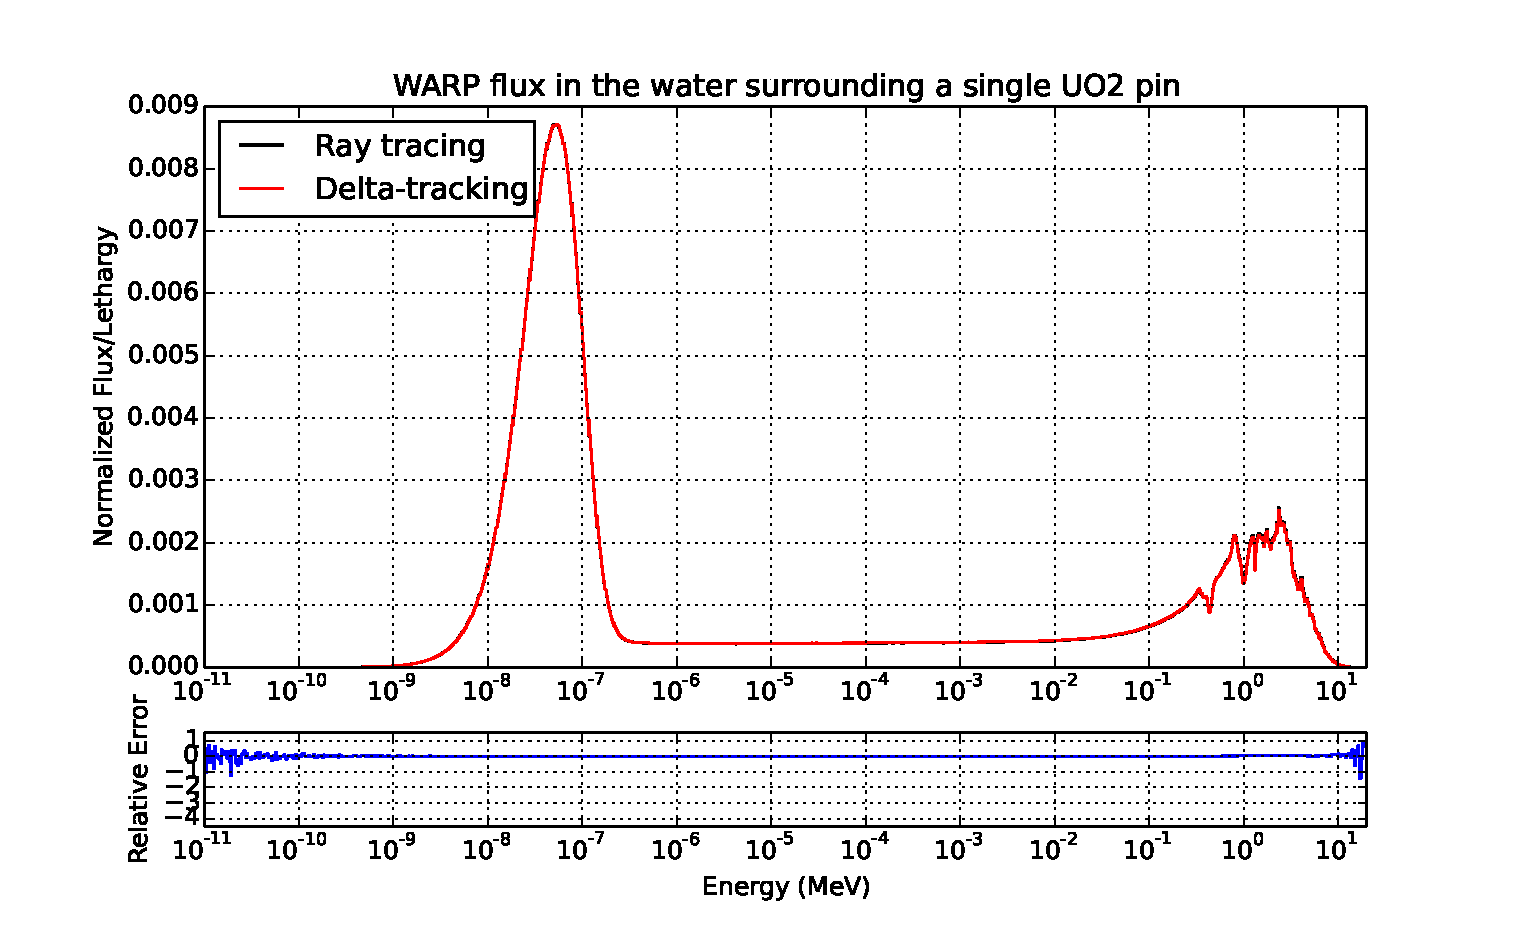
\includegraphics[width=\textwidth]{img/pincell-water.eps}
\caption{Normalized flux spectra for the \textbf{water} block in the pin cell configuration 
generated by both versions of WARP. \label{pincell-water}}
\end{figure}

In this basic, but heterogeneous, configuration, delta-tracking does not accurately calculate the 
multiplication factor for the system. Although the two values look similar, they do not match within
statistical uncertainty. Additionally, large discrepancies are seen in the neutron flux spectra in both
the fuel pin as well as the water surrounding it.

Figure \ref{pincell-fuel} shows that the flux spectrum in the fuel generated by the delta-tracking version
of WARP has slight but noticeable discrepancies compared to the flux spectrum generated by the original 
ray tracing version of the code. The fast and thermal flux are both underestimated, while the epithermal 
flux is overestimated. However, Figure \ref{pincell-water} shows that the flux spectrum in the water 
generated by the delta-tracking version matches the spectrum generated by ray tracing quite well. 

Note that the issues in the calculation of the effective multiplication factor and the normalized flux
spectrum in the fuel of the pin cell align. That is to say, there are more neutrons counted in the fuel in
the case of delta-tracking, and the overestimated value of $k_{\mathrm{eff}}$ also indicates greater 
numbers of neutrons than should actually be present. Since the spectral issue is only seen in the fuel 
(and the value of $k_{\mathrm{eff}}$ applies to the entire system), we may project that the original code 
perhaps has a bug in how fission events are handled. Since no fissions occur in the water, this could be a
potential source of the error seen above.

In this case, delta-tracking is again slower than ray tracing. The extra calculation time likely
comes from the calculation of the majorant at every instance of path length sampling as well as resampling
incurred by the use of the majorant in a system with multiple materials.

\subsection{Fuel pin assembly}

The ``fuel pin assembly" test consists of 631 $\ce{UO_2}$ cylinders arranged in a hexagonal lattice
surrounded by a cube of water with edges of length 84 cm. The material compositions and cylinder 
dimensions are identical to those described above in the pin cell case, but the large number of objects in
this scenario is intended to highlight the effect of introducing many geometric objects into a problem
\cite{warp2015}. Computational results for the fuel pin assembly configuration are shown in Table 
\ref{hex_table} and Figures \ref{assembly-centerpin} and \ref{assembly-water}.

\begin{table}[h!]
\centering
\caption{Calculated multiplication factors and runtimes for the fuel pin assembly configuration.}
\label{hex_table}
\begin{tabular}{| c | c | c |}
\hline
\textbf{Method} & $\mathbf{k_{\mathrm{eff}}}$ & \textbf{Runtime} \\
\hline
Ray tracing & $1.445201 \pm 2.3456 \times 10^{-4}$ & 4.36917 min \\
Delta-tracking & $1.415779 \pm 1.9934 \times 10^{-4}$ & 4.57683 min \\
\hline
\end{tabular}
\end{table}

\begin{figure}[h!]
\includegraphics[width=\textwidth]{img/assembly-centerpin.eps}
\caption{Normalized flux spectra for the \textbf{center pin} of a hexagonal array of $\ce{UO_2}$ 
pins in water generated by both versions of WARP. \label{assembly-centerpin}}
\end{figure}

\begin{figure}[h!]
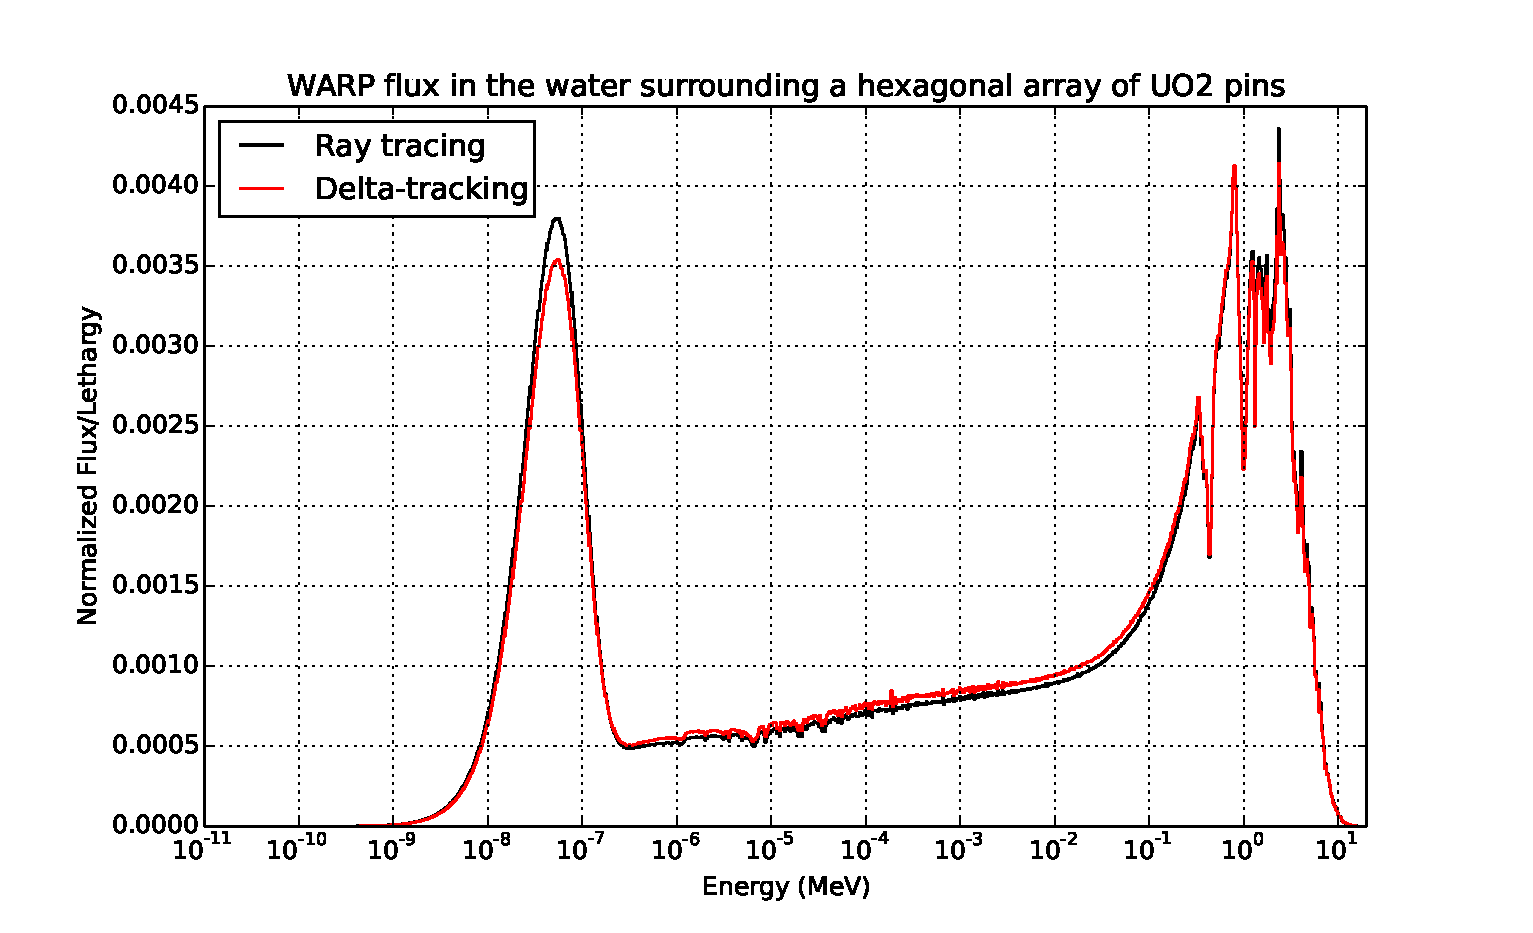
\includegraphics[width=\textwidth]{img/assembly-water.eps}
\caption{Normalized flux spectra for the \textbf{water} surrounding a hexagonal array of 
$\ce{UO_2}$ pins generated by both versions of WARP. \label{assembly-water}}
\end{figure}

The results for the fuel pin assembly simulation suffer from the same geometry issues discussed earlier
in the pin cell simulation results. Using the delta-tracking method causes the neutron multiplication
factor to be grossly underestimated. Spectral issues similar to those in the pin cell configuration are
observed; compared to the spectra generated using ray tracing, too many fast neutrons are in the center 
fuel pin in the assembly and too few thermal neutrons are in the water surrounding the fuel pins.
Given the mismatch in the single pin, this behavior is consistent with expectation.

In addition to these geometrical errors, the delta-tracking method is again slower than the ray tracing
algorithm. Computing the majorant cross section and resampling neutron interactions requires additional
runtime on top of the remainder of the Monte Carlo algorithm.

\section{Experimental homogeneous systems}
\label{sec:exp}

The discrepancies between the two methods in the results of the heterogenous systems prompted the
question of whether the incorrect behavior was caused by the implementation of the delta-tracking method 
or the original code as a whole. The homogeneous systems discussed above were not sufficient to answer 
this question as they contained only one outer boundary.

Taking these notions into consideration, a homogeneous system with artificial boundaries, shown below in 
Figure \ref{jezebel-shells}, was created to test the delta-tracking method against the ray tracing 
method once more. The material and geometry configuration is identical to the Jezebel configuration
described in Table \ref{test_setup} but with an artifical boundary inserted in the sphere. A more
extreme version of this configuration has four artificial boundaries and is shown in Figure 
\ref{jezebel-five}.

The configurations are obviously non-physical; they were contrived explicitly for the purpose of testing
the delta-tracking method in an environment more complex than the basic homogeneous systems in Section
\ref{sec:homog} but less complex than the full-blown heterogeneous configurations in Section 
\ref{sec:hetero}. From the results of these simulations we may infer that if the delta-tracking results
match those calculated with ray tracing, the issues observed in Section \ref{sec:hetero} are issues with
the code that already existed prior to the introduction of the delta-tracking method. If the results are
inconsistent, however, we may conclude that there is an error in the implementation of the delta-tracking
method.

\begin{figure}[h!]
\centering
\includegraphics[width=0.5\textwidth]{img/jezebel-shells.png}
\caption{Plot of ``Jezebel" configuration with an inserted artificial boundary. \label{jezebel-shells}}
\end{figure}

\begin{figure}[h!]
\centering
\includegraphics[width=0.5\textwidth]{img/jezebel-shells-five.png}
\caption{Plot of ``Jezebel" configuration with four artificial boundaries. \label{jezebel-five}}
\end{figure}

Results of simulations of the two experimental homogeneous systems follow in Tables 
\ref{jezebel_shells_table} and \ref{jezebel_five_table}. The results show that in each case, the
effective multiplication factor calculated using the delta-tracking method corresponds to that calculated
using the ray tracing method (within statistical error). It should be noted that the ray tracing method
referred to here is not the algorithm discussed in Section \ref{sec:rt} but the algorithm discussed in
Appendix \ref{app:A}. In testing these experimental homogeneous configurations, a major error was found
in the original ray tracing algorithm and it was replaced with a more correct method.

\begin{table}[h!]
\centering
\caption{Calculated multiplication factors and runtimes for the Jezebel configuration with one 
artificial boundary.}
\label{jezebel_shells_table}
\begin{tabular}{| c | c | c |}
\hline
\textbf{Method} & $\mathbf{k_{\mathrm{eff}}}$ & \textbf{Runtime} \\
\hline
Ray tracing* & $1.027356 \pm 3.4527 \times 10^{-4}$ & 20.29 s \\
Delta-tracking & $1.027218 \pm 2.7643 \times 10^{-4}$ & 23.79 s \\
\hline
\end{tabular}
\end{table}

\begin{table}[h!]
\centering
\caption{Calculated multiplication factors and runtimes for the Jezebel configuration with four 
artificial boundaries.}
\label{jezebel_five_table}
\begin{tabular}{| c | c | c |}
\hline
\textbf{Method} & $\mathbf{k_{\mathrm{eff}}}$ & \textbf{Runtime} \\
\hline
Ray tracing* & $1.027238 \pm 2.7643 \times 10^{-4}$ & 24.27 s \\
Delta-tracking & $1.027425 \pm 2.7085 \times 10^{-4}$ & 24.06 s \\
\hline
\end{tabular}
\end{table}

Again, the runtimes of the two methods are comparable, with the delta-tracking method actually outpacing
the new ray tracing algorithm for the case of the Jezebel configuration with four artificial boundaries.
Because the delta-tracking method is consistent with ray tracing for the cases of configurations with a
single material and multiple cells, we may infer that the issues seen in Section \ref{sec:hetero} are due
to exacerbation of preexisting bug(s) in the code by the delta-tracking method. As a result, one cannot
determine whether or not delta-tracking is a viable neutron tracking routine for good performance on GPUs.
However, the performance of the routine observed in the experimental homogeneous cases above indicates the
potential of the delta-tracking method on GPUs.

\chapter{Conclusions and Future Work}

\section{Conclusions}

In this work, delta-tracking was implemented as a neutron tracking routine in a GPU-accelerated Monte
Carlo neutron transport code and the results were compared for accuracy and speed with respect to the 
original ray tracing version of the code. For systems comprised solely of a homogeneous material, the
delta-tracking method produced results consistent to within statistical uncertainty of those calculated
using ray tracing. The delta-tracking method failed to achieve consistent results when simulating
heterogeneous systems, however. Further testing of homogeneous systems with artificial boundaries in 
place revealed that those boundaries do not skew the results of the delta-tracking routine such that they
are outside of the level expected. Thus, it may be concluded that there are existing bugs in the
original ray tracing version of the code that the delta-tracking routine exacerbates, causing results
from the latter method to be incorrect.

The speeds of the two physics methods were comparable, with ray tracing often slightly faster than 
delta-tracking. The relative lag of the delta-tracking method can be easily explained by the fact that it
requires an additional OptiX trace in addition to the single trace required by ray tracing. However, since
 the runtimes of both methods were fairly close we assert that, for configurations with many cells, the
homogenization of the delta-tracking may mitigate the effect of the slowdown from the second trace, 
allowing it to perform better than ray tracing.

However, before further scaling studies can be done with the delta-tracking method, the original core of
the code must be closely examined to resolve existing bugs. After the prevalent issues have been solved,
delta-tracking may be revisited.

\section{Future Work}

The first point of future work is to resolve the issues in the existing ray tracing code. This will be
done in several thrusts. Work is planned to reorganize the main data structures in the code such that
they are simpler, more intuitive, and more easily understood by interested developers new to the code.
Additionally, more unit testing in the code will provide useful information about the functionality of the individual CUDA kernels. If it is known that all individual kernels are functioning as expected, it 
follows that the code as a whole should function as expected as well.

Once the core of the WARP code has been restructured and unit tests implemented such that WARP is more
robust and correct, delta-tracking may be revisited. The implementation discussed here should be tested
against the fixed code to verify correctness and measure speed. If this delta-tracking method is still
slower than ray tracing for the majority of configurations, an alternative algorithm may be developed. 
The OptiX framework may be leveraged to provide the information needed for the delta-tracking method
using only one trace, which could allow delta-tracking to perform better than ray tracing.



\begin{appendix}
\chapter{New ``Where Am I" Algorithm}
\label{app:A}

This appendix includes a disscussion of the new particle location and material update (``where am I")
algorithm in the WARP code. The discussion is included here as an appendix because this algorithm was 
updated after the original presentation corresponding to the master's degree and this report.

The original algorithm, discussed in Section \ref{sec:rt}, was found to produce incorrect results when 
testing the experimental material and geometry configurations discussed in Section \ref{sec:exp}.
Because of this, the particle location update algorithm was modified to be able to
correctly handle such configurations in addition to the ones originally tested.

WARP now uses ``cell sense" in its ray tracing implementation to determine in which cell and material a
neutron is located. Cell sense is positive if a neutron is outside of a cell and negative if a neutron is
inside of a cell; it is the product of the surface senses of the cell's constituent planes. Figure 
\ref{whereaminew} shows an illustration of the process.

\begin{figure}[h!]
\centering
\includegraphics[width=0.9\textwidth]{img/whereami-new.pdf}
\caption{The new, improved point-in-polygon ``where am I" algorithm. \label{whereaminew}}
\end{figure}

In WARP, the surface normal vectors always point outward and the signs of the normals encountered along a
trace are summed in the tracing process. When the sum becomes negative, the trace is stopped, and the 
last intersected cell (and its corresponding material) is the one in which the neutron is located.

Previously, a list of cell numbers was stored for each cell surface intersection that occurred along the
trace with the double entries removed to make a nested list of the cell(s) in which a neutron was 
located. In the new algorithm, cell sense is calculated on the fly as the query ray traverses the
configuration geometry, allowing the trace to stop as soon as the cumulative sense becomes negative. This
is possible because WARP requires that all geometry surfaces be closed. Additionally, compared to the
prior scheme of storing and operating on a list of integers, this new method only requires a single 
integer to be stored and operated on.

\end{appendix}

\printbibliography

\end{document}
